\documentclass{article}
\usepackage{dot2texi}
\usepackage{tikz}
\usetikzlibrary{shapes,arrows}
\begin{document}
\begin{figure}
	\centering
	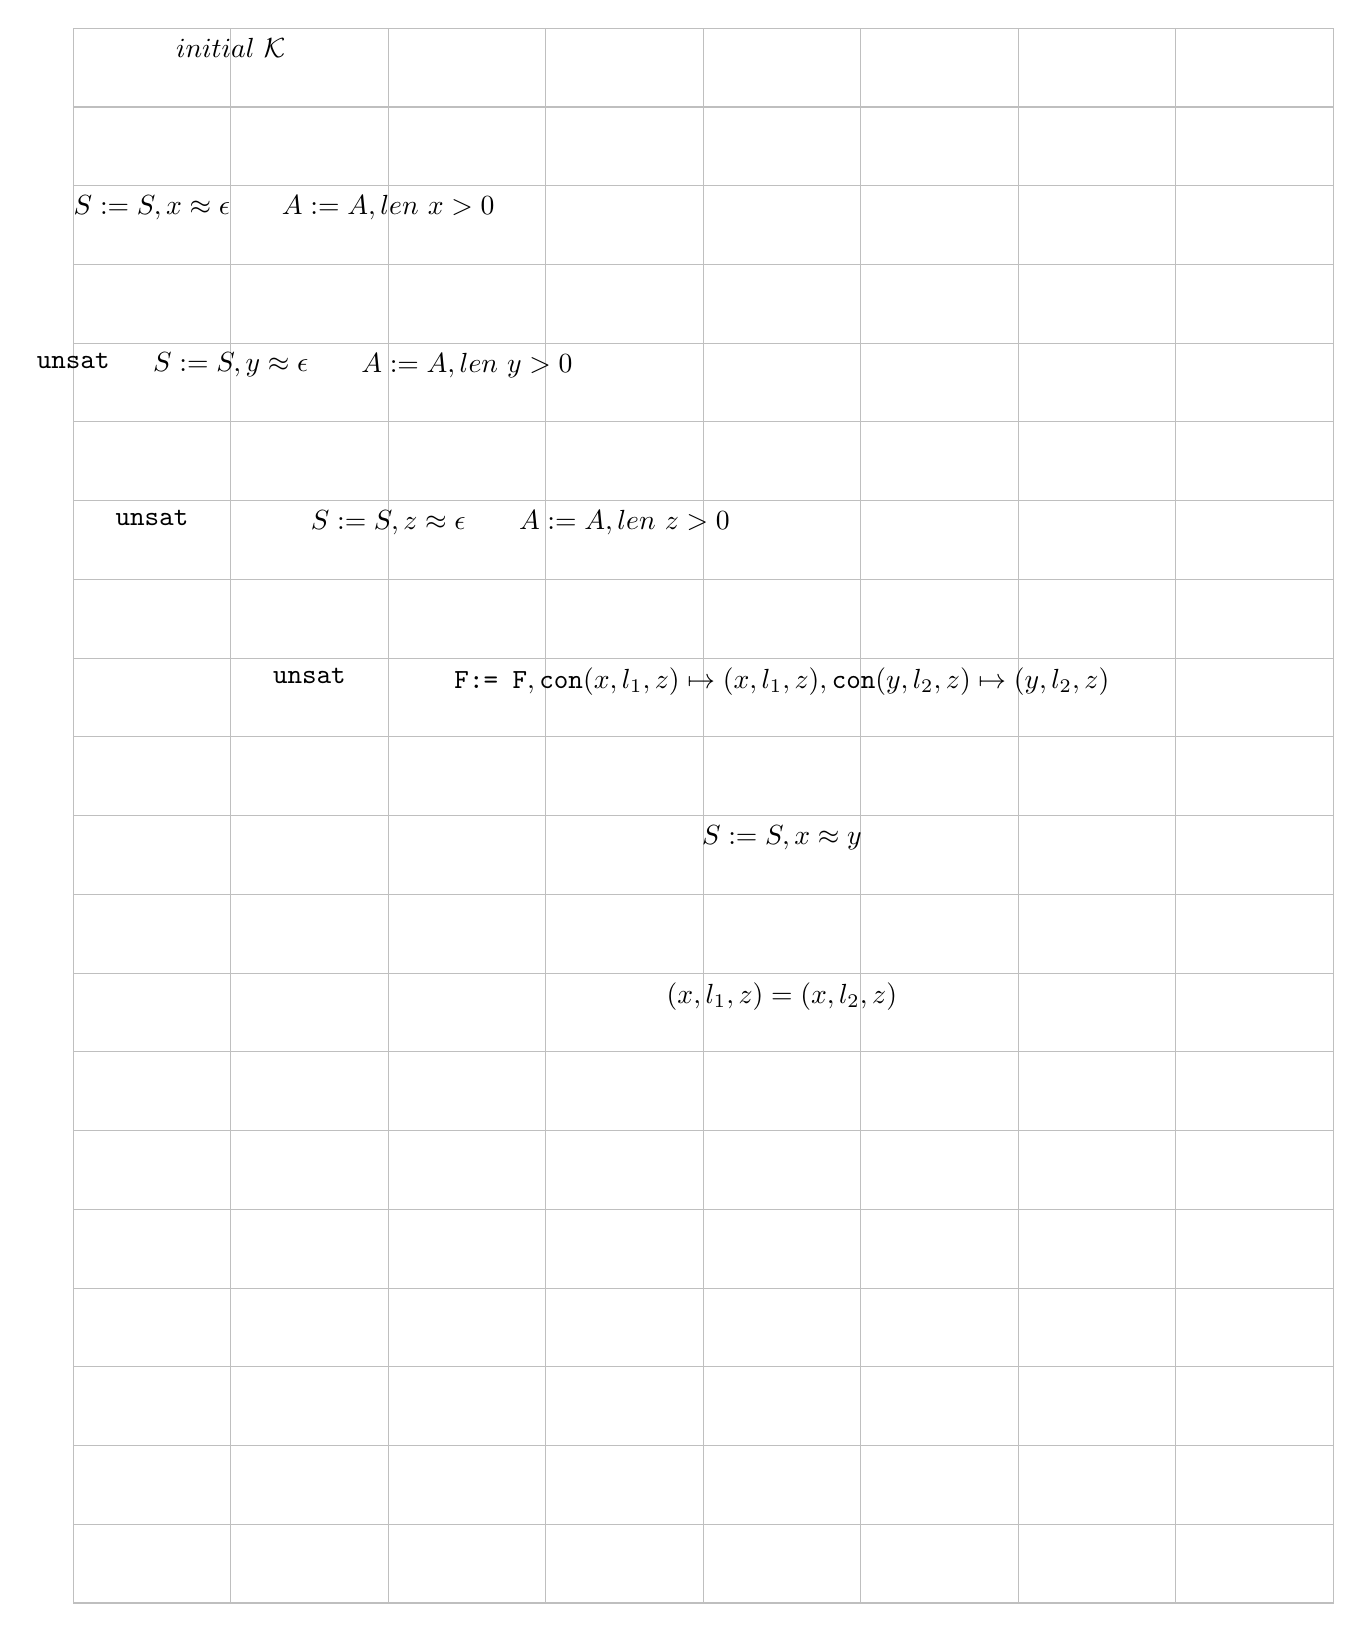
\begin{tikzpicture}
	\draw [lightgray](0,0) --(0,20) -- (16,20)-- (16,0) --(0,0);
	\draw [lightgray](0,1) --(16,1);
	\draw [lightgray](0,2) --(16,2);
	\draw [lightgray](0,3) --(16,3);
	\draw [lightgray](0,4) --(16,4);
	\draw [lightgray](0,5) --(16,5);
	\draw [lightgray](0,6) --(16,6);
	\draw [lightgray](0,7) --(16,7);
	\draw [lightgray](0,8) --(16,8);
	\draw [lightgray](0,9) --(16,9);
	\draw [lightgray](0,10) --(16,10);
	\draw [lightgray](0,11) --(16,11);
	\draw [lightgray](0,12) --(16,12);
	\draw [lightgray](0,13) --(16,13);
	\draw [lightgray](0,14) --(16,14);
	\draw [lightgray](0,15) --(16,15);
	\draw [lightgray](0,16) --(16,16);
	\draw [lightgray](0,17) --(16,17);
	\draw [lightgray](0,18) --(16,18);
	\draw [lightgray](0,19) --(16,19);
	\draw [lightgray](0,20) --(16,20);
	
	\draw [lightgray](2, 0) --(2,20);
	\draw [lightgray](4, 0) --(4,20);
	\draw [lightgray](6, 0) --(6,20);
	\draw [lightgray](8, 0) --(8,20);
	\draw [lightgray](10, 0) --(10,20);    
	\draw [lightgray](12, 0) --(12,20);
	\draw [lightgray](14, 0) --(14,20);

	\node [below] at (2,20) {$ initial \ \mathcal{K}$};
	
	\node [below] at (1,18) {$S:=S, x\approx \epsilon$};
	\node [below] at (4,18) {$A:=A, len \ x  > 0$};
	
	\node [below] at (0,16) {$\texttt{unsat}$};
	\node [below] at (2,16) {$S:=S, y\approx \epsilon$};
	\node [below] at (5,16) {$A:=A, len \ y  > 0$};
	
	\node [below] at (1,14) {$\texttt{unsat}$};
	\node [below] at (4,14) {$S:=S, z\approx \epsilon$};
	\node [below] at (7,14) {$A:=A, len \ z  > 0$};
	
	\node [below] at (3,12) {$\texttt{unsat}$};
	\node [below] at (9,12) {$\texttt{F:= F},\texttt{con}(x,l_1,z)\mapsto (x,l_1,z),\texttt{con}(y,l_2,z)\mapsto(y,l_2,z)$};
	
	\node [below] at (9,10) {$S:=S, x\approx y$};
	
	\node [below] at (9,8) {$( x, l_1, z ) = (x, l_2,z)$};
	
	
	
	
	
	\end{tikzpicture}
	\caption{The derivation tree for example 1.}
\end{figure}	
	
	
	
\begin{figure}
	\centering	
	\begin{dot2tex}[mathmode]
		digraph G {
			rankdir=TB;
			node [shape=box];
			root [texlbl="$initial \mathcal{K}$"];
			a [texlbl="$S:=S, x \approx \epsilon$"];
			b [texlbl="$A:=A, \texttt{len} \ x >0$"];
			
			root:left -> a [texlbl="$Len-Split$",style=bold,label="100 times"];
			root:right -> b [texlbl="$Len-Split$",style=bold,label="100 times"];
			
			
			label="Graph label $\approx$";
			lblstyle="draw,fill=red!20";
			
		};		
	\end{dot2tex}
	\caption{derivation tree}
\end{figure}	
	
\begin{figure}
\centering	
\begin{dot2tex}[mathmode]
digraph G{
	node [shape="box"];
	root [texlbl="$initial\  \mathcal{K}$"];
	a [texlbl="$a$"];
	b [texlbl="$b$"];
	c [texlbl="$c$"];
	d [texlbl="$d$"];
	root:left -> a  [style=bold,label="100 times"];
	root:right -> b;
	a:left -> c;
	a:right -> d;    
}
\end{dot2tex}
\caption{derivation tree}
\end{figure}

\begin{tikzpicture}[
grow=down,
level 1/.style={sibling distance=3.5cm,level distance=2.2cm},
level 2/.style={sibling distance=3.5cm, level distance=2.2cm},
edge from parent/.style={draw=gray},
edge from parent path={(\tikzparentnode.south) -- (\tikzchildnode.north)},
kant/.style={text width=2cm},
every node/.style={text ragged, inner sep=2mm},
punkt/.style={rectangle, top color=white, bottom color=white, draw=black }
]
\draw [lightgray](0,0) --(0,20) -- (16,20)-- (16,0) --(0,0);
\draw [lightgray](0,1) --(16,1);
\draw [lightgray](0,2) --(16,2);
\draw [lightgray](0,3) --(16,3);
\draw [lightgray](0,4) --(16,4);
\draw [lightgray](0,5) --(16,5);
\draw [lightgray](0,6) --(16,6);
\draw [lightgray](0,7) --(16,7);
\draw [lightgray](0,8) --(16,8);
\draw [lightgray](0,9) --(16,9);
\draw [lightgray](0,10) --(16,10);
\draw [lightgray](0,11) --(16,11);
\draw [lightgray](0,12) --(16,12);
\draw [lightgray](0,13) --(16,13);
\draw [lightgray](0,14) --(16,14);
\draw [lightgray](0,16) --(16,16);
\draw [lightgray](0,16) --(16,16);
\draw [lightgray](0,17) --(16,17);
\draw [lightgray](0,18) --(16,18);
\draw [lightgray](0,19) --(16,19);
\draw [lightgray](0,20) --(16,20);

\node[punkt, text width=5.5em] {$initial\ \mathcal{K}$}
%Lower part lv1
child {
	node[punkt] [rectangle split, rectangle split, rectangle split parts=1,
	text ragged] { $\texttt{S:= S},x\approx\epsilon$  }
	child{
		node { $\texttt{unsat}$}
		edge from parent node[kant, above, pos=.6] {$\texttt{A-Conflict}$}
	}                    
	edge from parent
	node[kant] {$\texttt{Len-Split}$}
    
}
child {
	node[punkt] [rectangle split, rectangle split, rectangle split parts=1,text ragged] { $\texttt{A:= A},\texttt{len}\ x > 0$  }
	child {
		node[punkt] [rectangle split, rectangle split, rectangle split parts=1,text ragged] { $\texttt{S:= S},z\approx\epsilon$  }
		child{
			node { $\texttt{unsat}$}
			edge from parent node[kant, above, pos=.6] {$\texttt{A-Conflict}$}
		}
		edge from parent node[kant, below, pos=.6] {$\texttt{Len-Split}$}
	}
	child {
		node[punkt] [rectangle split, rectangle split, rectangle split parts=1,text ragged] { $\texttt{A:= A},\texttt{len}\ z > 0$  }
		child{
			node[punkt] [rectangle split, rectangle split, rectangle split parts=1,text ragged] { $\texttt{S:= S},y\approx\epsilon$  }
			child{
				node { $\texttt{unsat}$}
				edge from parent node[kant, above, pos=.6] {$\texttt{A-Conflict}$}
			}
			edge from parent node[kant] {$\texttt{Len-Split}$}
		}
		child{
			node[punkt] [rectangle split, rectangle split, rectangle split parts=1,text ragged] {$\texttt{A:= A},\texttt{len}\ y > 0$}
			child{
				node[punkt] [rectangle split, rectangle split, rectangle split parts=1,text ragged] {$\texttt{F:= F},con(x,l_1,z)\mapsto (x,l_1,z),con(y,l_2,z)\mapsto(y,l_2,z)$}
				edge from parent node[kant] {$\texttt{N-Form2,F-Form2,N-Form1,F-Form1}$}
			}                  
			edge from parent node[kant] {$\texttt{Len-Split}$}
		}
		edge from parent node[kant, below, pos=.6] {$\texttt{Len-Split}$}
	}            
	edge from parent node[kant, below, pos=.6] {$\texttt{Len-Split}$}
}
\node [below] at (10,9.6) {$\texttt{Len-Split}$};

\draw [->] (10,9.3) -- (8,8.5);
\draw [->] (10,9.3) -- (12,8.5);


\draw [->] (5,5) -- (4,4.5);
\node [right] at (2,8) {$\texttt{F:= F},\texttt{con}(x,l_1,z)\mapsto (x,l_1,z),\texttt{con}(y,l_2,z)\mapsto(y,l_2,z)$};
\node [right] at (6,7.2) {$\texttt{F-Unify}$};
\draw [->] (6,7.8) -- (6,6.8);
\node [right] at (5,6.5) {$\texttt{S:= S},x\approx y$};

%Upper part, lv1
;
\end{tikzpicture}
\end{document}
